\documentclass{book}
\usepackage[utf8]{inputenc}
\usepackage{pgfplots}
\pgfplotsset{compat=1.6}
\begin{document}

\begin{figure}
  \centering
  
  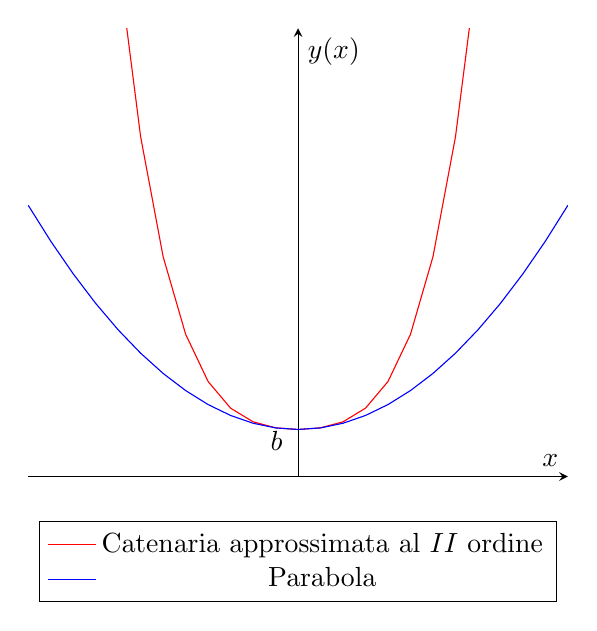
\begin{tikzpicture}
    \begin{axis}[
      legend style = {at= {(0.5,-.1)}, anchor = north},
      axis x line = center,
      axis y line = center,
      xlabel=$x$,
      ylabel=$y(x)$,
      xtick=\empty,
      ytick=\empty,
      ymin=0, 
      xmin = -5, 
      xmax = 5,
      ymin= 0,
      ymax=100,
      ytick = {10.5},
      yticklabel = $b$,
      yticklabel style = {yshift = -.15cm}
      ]

\addplot[draw, red] {10.5+2*\x*\x + (1/24)*16*(\x)^4};
\addlegendentry{Catenaria approssimata al $II$ ordine};

\addplot[draw, blue] {10.5 + 2*\x*\x };
\addlegendentry{Parabola};
    \end{axis}

  \end{tikzpicture}
   
  
 \end{figure}






\end{document}
